\documentclass{article}[11pt]

\usepackage{Geoff,graphicx}

\begin{document}
\title{DFC 2018 dataset}
\author{Geoffrey Iyer}
\maketitle

We recently got our hands on the dataset for the 2018 Data Fusion Contest. Here are some brief notes about it.

\section{DFC 2018 dataset}

This is multi-source remote sensing data of an urban neighborhood. The goal of the contest is ``urban land use and land cover classification''. The dataset consists of.
\begin{itemize}
\item Multispectral lidar at a resolution of 0.5m ground sampling distance
\item Hyperspectral data (50 bands) at 1m resolution
\item Very high resolution RFG at 5cm resolution
  \item Ground truth data (21 classes) for the whole region at 0.5m resolution.
\end{itemize}

The size of the hyperspectral data is roughly 1.4 million pixels. So the lidar is $4\times$ that and the RGB is... quite big. See the figures for a few selected images of the data.

\begin{figure}
  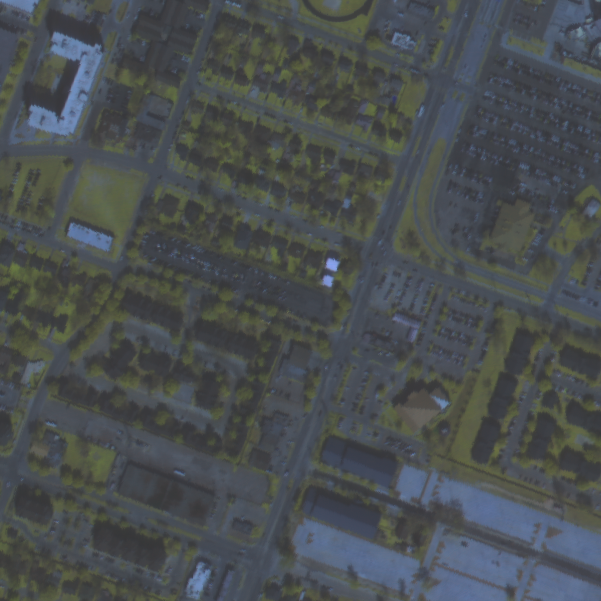
\includegraphics[width=\linewidth]{Hyperspectral.png}
  \caption{RGB bands from Hyperspectral data}
\end{figure}

\begin{figure}
  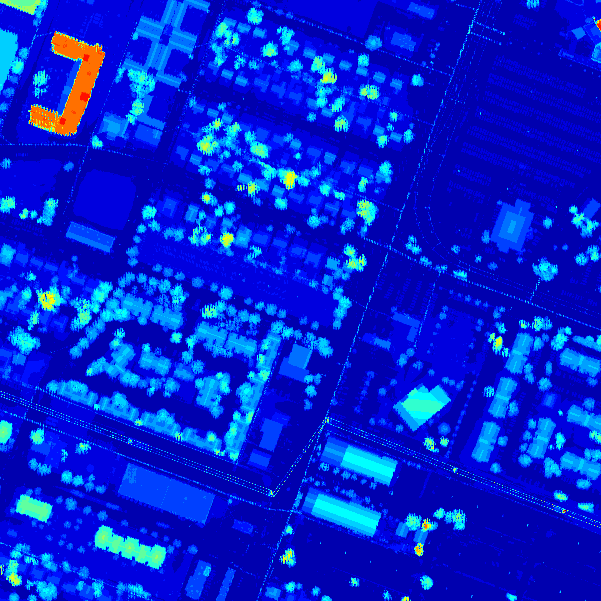
\includegraphics[width=\linewidth]{lidar4.png}
  \caption{One selected band from lidar data}
\end{figure}

\begin{figure}
  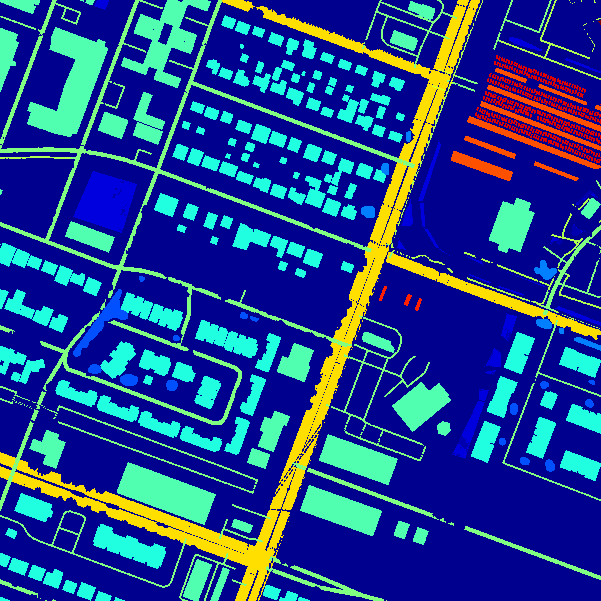
\includegraphics[width=\linewidth]{Ground_Truth.png}
  \caption{Ground truth}
\end{figure}

\section{First results on the data}

I haven't had the time to do much with this yet. So far I've only run spectral clustering on this set, using the multimodal weights as in our paper. It took some time because my original code was only built to handle 2 modalities (in hindsight this was pretty silly). See the figures for some basic results.

To deal with the differences in resolution, I reduced the lidar to the same size as the hyperspectral, and I didn't use the RGB at all. For spectral clustering, I chose to use 6 classes. There isn't any real reason behind the number 6. I just wanted to see some preliminary results.

\begin{figure}
  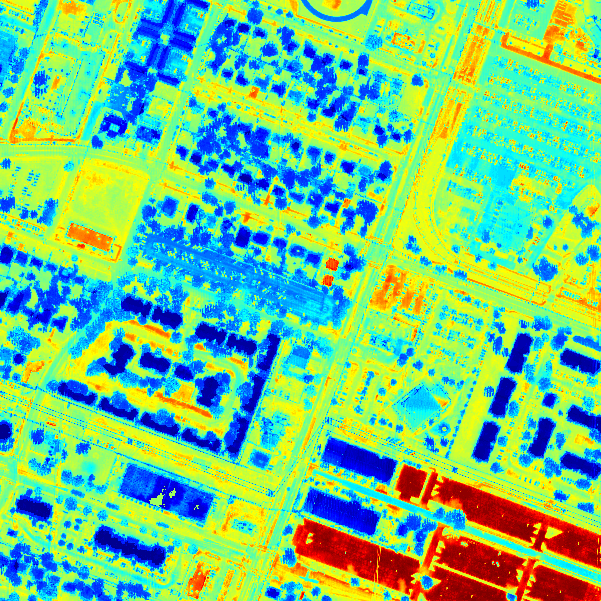
\includegraphics[width=\linewidth]{evec1.png}
  \caption{Example eigenvector 1}
\end{figure}

\begin{figure}
  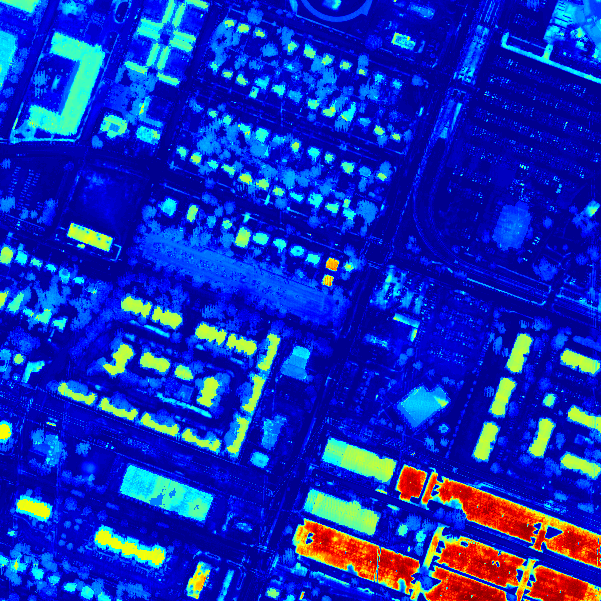
\includegraphics[width=\linewidth]{evec2.png}
  \caption{Example eigenvector 2}
\end{figure}

\begin{figure}
  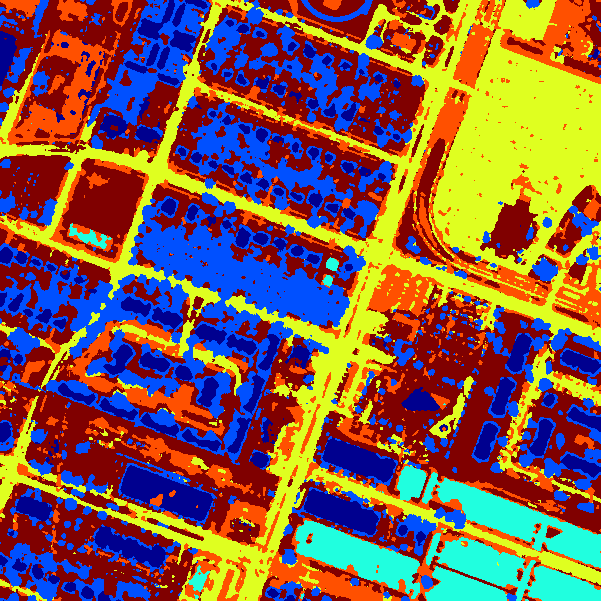
\includegraphics[width=\linewidth]{specClust4Norm.png}
  \caption{Spectral Clustering result}
\end{figure}

\section{Next Steps}

I'm pretty excited to get access to this dataset, as this is much more ``multimodal'' than anything we've worked with before. If we can get even some basic results here I think it'll improve our image segmentation/classification paper a lot. One restriction is the size of the data. At the resolution of the Hyperspectral image it's already quite big. The lidar images are worse, and I think the RGB is out of the question.

The obvious next step is to run this through MBO. Once again this is going to take some coding because I currently have it running only 2 modalities (whoops). Then depending on how that look we can think about how to move forward.

\end{document}